%%%%%%%%%%%%%%%%%%%%%%%%%%%%%%%%%%%%%%%
% Deedy CV/Resume
% XeLaTeX Template
% Version 1.0 (5/5/2014)
%
% This template has been downloaded from:
% http://www.LaTeXTemplates.com
%
% Original author:
% Debarghya Das (http://www.debarghyadas.com)
% With extensive modifications by:
% Vel (vel@latextemplates.com)
%
% License:
% CC BY-NC-SA 3.0 (http://creativecommons.org/licenses/by-nc-sa/3.0/)
%
% Important notes:
% This template needs to be compiled with XeLaTeX.
%
%%%%%%%%%%%%%%%%%%%%%%%%%%%%%%%%%%%%%%

\documentclass[letterpaper]{my-resume} % Use US Letter paper, change to a4paper for A4 

\usepackage{graphicx} % Picture
\usepackage[absolute]{textpos} % Picture + QRCode
\usepackage{verbatim} % Multiline comments 

%\begin{comment}
%\end{comment}

\begin{document}

\begin{textblock}{2.5}(5,2)
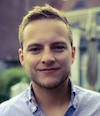
\includegraphics[scale=0.75]{profil.jpg}
\end{textblock}

\begin{textblock}{2.5}(78,4)

\includegraphics[scale=0.30]{qrcode.png}
\end{textblock}

%----------------------------------------------------------------------------------------
%	TITLE SECTION
%----------------------------------------------------------------------------------------

\lastupdated % Print the Last Updated text at the top right

\namesection{Maxime}{Hardy}{ % Your name
\urlstyle{same}\url{http://hardy.im} \\ % Your website, LinkedIn profile or other web address
\textbf{Jnr. Front-End Web Developer} \\
\href{mailto:maxime@hardy.lu}{maxime@hardy.lu} | (+44) 07783 126066 \\ % Your contact information
}

%----------------------------------------------------------------------------------------
%	LEFT COLUMN
%----------------------------------------------------------------------------------------

\begin{minipage}[t]{0.33\textwidth} % The left column takes up 33% of the text width of the page

%------------------------------------------------
% Education
%------------------------------------------------

\section{Education} 

\begin{comment}

\subsection{Cornell University}

\descript{MEng in Computer Science}
\location{Expected Dec 2014 | Ithaca, NY \\ Cum. GPA: N/A}

\sectionspace % Some whitespace after the section

\descript{BS in Computer Science}
\location{Expected May 2014 | Ithaca, NY}
Conc. in Software Engineering \\
College of Engineering \\
Dean's List (All Semesters) \\
\location{ Cum. GPA: 3.92 / 4.0 \\
Major GPA: 3.94 / 4.0}

\sectionspace % Some whitespace after the section

\end{comment}

%------------------------------------------------

\subsection{Stafford House School}

\location{Expected Apr 2016 | London, UK \\ Final lvl: B2/C1}

\descript{Business English and general English lessons}

\sectionspace % Some whitespace after the section

%------------------------------------------------

\subsection{Institute Paul Lambin}

\location{Expected June 2015 | Brussels, BE \\ Cum. GPA: 71,83\%}

\descript{BSc with Distinction in information technology}

\sectionspace % Some whitespace after the section

%------------------------------------------------

\subsection{Uni. libre de Bruxelles}

\location{2010 - 2012 | Brussels, BE \\ Cum. GPA: N/A}

\descript{Preparatory training in computer science}

\sectionspace % Some whitespace after the section

%------------------------------------------------

%\begin{comment}

\subsection{Institute Saint-Louis}

\location{Expected Dec 2010 | Brussels, BE \\ Cum. GPA: N/A}

\descript{Mathematics courses}

\sectionspace % Some whitespace after the section

%\end{comment}

%------------------------------------------------
% Links
%------------------------------------------------

\section{Links} 

Mail:// \href{mailto:maxime@hardy.lu}{\bf maxime@hardy.lu} \\
LinkedIn:// \href{https://www.linkedin.com/in/maximehardy}{\bf maximehardy} \\
Website:// \href{http://hardy.im}{\bf hardy.im} \\
Github:// \href{https://github.com/mxhuk}{\bf mxhduk} \\
\begin{comment}
Twitter:// \href{https://twitter.com/mxhduk}{\bf @mxhduk} \\
Quora:// \href{https://www.quora.com/mxhduk}{\bf mxhduk}
\end{comment}

\sectionspace % Some whitespace after the section

%------------------------------------------------
% Skills
%------------------------------------------------

\section{Skills}

\subsection{Programming}

\location{Over 5000 lines:}
Java \textbullet{} Shell \textbullet{} JavaScript \textbullet{} Matlab \\
OCaml \textbullet{} Python \textbullet{} Rails \textbullet{} \LaTeX\ \\ 
\location{Over 1000 lines:}
C \textbullet{} C++ \textbullet{} CSS \textbullet{} PHP \textbullet{} Assembly \\
\location{Familiar:}
AS3 \textbullet{} iOS \textbullet{} Android \textbullet{} MySQL

\sectionspace % Some whitespace after the section

%------------------------------------------------
% Additional
%------------------------------------------------

\section{Additional}

\subsection{About}

Brussels, Belgium \\
9 August 1991 

\sectionspace % Some whitespace after the section

%------------------------------------------------

\subsection{Languages}

\textbf{French} - Native \\
\textbf{English} - B2/C1 \\
\textbf{Dutch} - A1

\begin{comment}

{\footnotesize \textit{\textbf{(Research Asst. \& Teaching Asst) }}}

\end{comment}

\sectionspace % Some whitespace after the section

%----------------------------------------------------------------------------------------

\end{minipage} % The end of the left column
\hfill
%
%----------------------------------------------------------------------------------------
%	RIGHT COLUMN
%----------------------------------------------------------------------------------------
%
\begin{minipage}[t]{0.66\textwidth} % The right column takes up 66% of the text width of the page

%------------------------------------------------
% Experience
%------------------------------------------------

\section{Experience}

\begin{comment}

\runsubsection{Coursera}
\descript{| KPCB Fellow + Software Engineering Intern}

\location{Expected June 2014 ? Sep 2014 | Mountain View, CA}
\vspace{\topsep} % Hacky fix for awkward extra vertical space
\begin{tightitemize}
\item 52 out of 2500 applicants chosen to be a KPCB Fellow 2014.
\end{tightitemize}

\sectionspace % Some whitespace after the section

\end{comment}

%------------------------------------------------

\runsubsection{Agilos}
\descript{| 4-month internship as Jnr. Technical Consultant BI}

\location{Expected Feb 2015 ? June 2015 | Brussels, BE}
\vspace{\topsep} % Hacky fix for awkward extra vertical space
\begin{tightitemize}
\item In-depth comparison between QlikView and QlikSense.
\item (Re)develop a QlikView/QlikSense application (also include mobile, extensions, geographical ... sides).
\item I developed some experience in presenting through Agilos internal workshops.
\end{tightitemize}

\sectionspace % Some whitespace after the section

%------------------------------------------------

\runsubsection{Worldline}
\descript{| Short internship as observer}

\location{Expected Feb 2014 (5 days) | Brussels, BE}
%\vspace{\topsep} % Hacky fix for awkward extra vertical space
\begin{tightitemize}
\item Understanding company processus and more precisely the IT department.
\item Real approach of subject school.
\end{tightitemize}

\sectionspace % Some whitespace after the section

%------------------------------------------------

\runsubsection{Institute Jules Bordet}
\descript{| Front-End dev, ba, training}

\location{Expected Feb 2012 ? Apr 2012 | Brussels, BE}
%\vspace{\topsep} % Hacky fix for awkward extra vertical space
\begin{tightitemize}
\item Development of a web platform for the urology department.
\item All the Front-End part and only the analysis of Back-End.
\item Analysis of the business requirements + Meetings with the different stakeholders.
\end{tightitemize}

\sectionspace % Some whitespace after the section

%------------------------------------------------
% Projects
%------------------------------------------------

\section{Projects}

\begin{comment}

\runsubsection{Cornell Robot Learning Lab}
\descript{| Head Undergrad Research}

\location{Jan 2014 ? Present | Ithaca, NY}
Worked with \textbf{\href{http://www.cs.cornell.edu/~ashesh/}{Ashesh Jain}} and \textbf{\href{http://www.cs.cornell.edu/~asaxena/}{Prof Ashutosh Saxena}} to create \textbf{PlanIt}, a tool which learns from large scale user preference feedback to plan robot trajectories in human environments. Publication submitted.

\sectionspace % Some whitespace after the section

\end{comment}

%------------------------------------------------

\runsubsection{Mwsik - Music Social Network}
\descript{| Front-End \& Back-End dev}

\location{Oct 2015 ? Dec 2015 | Brussels, BE}
Lorem ipsum dolor sit amet, consectetur adipiscing elit. Duis quis suscipit mi. Pellentesque condimentum, enim ut ullamcorper facilisis, diam magna ultrices metus, eu interdum tortor est in est. Aliquam vulputate magna risus, in consectetur quam sollicitudin et.

\sectionspace % Some whitespace after the section

%------------------------------------------------

\runsubsection{Private project - Search Engine}
\descript{| Front-End dev, advertising placement and SEO analysis}

\location{May 2012 ? May 2013 | Brussels, BE}
The project aimed to creat a search engine with more than \textbf{2,000,000 articles} indexed. The website is still online and the content is automatically scrapped. The regular traffic was \textbf{15,000 visitors} a day. I participated in all of Front-End development, advertising placement and SEO optimization. At the same time we created URL shortener to support advertising placement optimisation.

\sectionspace % Some whitespace after the section

%------------------------------------------------

\runsubsection{Private project - Video library website}
\descript{| Front-End dev, Back-End and database structure analysis}

\location{Nov 2011 ? Apr 2012 | Brussels, BE}
The purpose of this website was to create a platform of indexed movies and TV show?s. The information about the movies was scrapped automatically on different sources. The regular traffic was 5,000 visitors a day. It was my first big personal project.

\sectionspace % Some whitespace after the section

%------------------------------------------------
% Awards
%------------------------------------------------

\begin{comment}

\section{Awards} 

\begin{tabular}{rll}
2014	 & top 52/2500 & KPCB Engineering Fellow\\
2014	 & 2\textsuperscript{nd} most points & Google Code Jam, Qualification Round\\
2014	 & 1\textsuperscript{st}/50 & Microsoft Coding Competition, Cornell\\
2013	 & National & Jump Trading Challenge Finalist\\
2013 & 7\textsuperscript{th}/120 & CS 3410 Cache Race Bot Tournament \\
2012 & 2\textsuperscript{nd}/150 & CS 3110 Biannual Intra-Class Bot Tournament \\
2011 & National & Indian National Mathematics Olympiad (INMO) Finalist \\
2010 & National & Comp. Soc. of India's National Programming Contest\\
\end{tabular}

\sectionspace % Some whitespace after the section

\end{comment}

%----------------------------------------------------------------------------------------

\end{minipage} % The end of the right column

%----------------------------------------------------------------------------------------
%	SECOND PAGE (EXAMPLE)
%----------------------------------------------------------------------------------------

%\newpage % Start a new page

%\begin{minipage}[t]{0.33\textwidth} % The left column takes up 33% of the text width of the page

%\section{Example Section}

%\end{minipage} % The end of the left column
%\hfill
%\begin{minipage}[t]{0.66\textwidth} % The right column takes up 66% of the text width of the page

%\section{Example Section 2}

%\end{minipage} % The end of the right column

%----------------------------------------------------------------------------------------

\end{document}